\documentclass[aspectratio=1610]{beamer}
\usepackage[utf8]{inputenc}
\usepackage{ragged2e}
\usepackage{xcolor}
\usepackage[italian]{babel}
\usetheme[progressbar=frametitle,titleformat=smallcaps]{metropolis}
\setbeamertemplate{frame numbering}[fraction]
\setbeamercovered{dynamic}
\definecolor{rosso}{RGB}{255, 0, 0}
\definecolor{giallo}{RGB}{254,212,23}
\hypersetup{colorlinks=true,linkcolor=black,urlcolor=rosso}
\setbeamercolor{palette primary}{fg=black, bg=giallo}
\setbeamercolor{background canvas}{bg=white}
\setbeamercolor{normal text}{fg=black}
\setbeamercolor{progress bar}{fg=rosso}
\setbeamercolor{framesubtitle}{fg=rosso}
\setbeamercolor{normal text .dimmed}{fg=giallo}
\setbeamercolor{block title alerted}{fg=rosso, bg=giallo}
\setbeamerfont{caption}{size=\tiny}
\setbeamerfont{caption name}{size=\tiny}
\setlength{\abovecaptionskip}{0pt}
\makeatletter
\metroset{block=fill}
\setlength{\metropolis@progressinheadfoot@linewidth}{1pt} 
\setlength{\metropolis@progressonsectionpage@linewidth}{1pt}
\setlength{\metropolis@titleseparator@linewidth}{1pt}
\makeatother

\title{TRASMISSIONE DATI}
\subtitle{mezzi e modalità di trasmissione}
\date{}
\institute{\textit{
        Fonti:
        \begin{itemize}
            \item[-] \href{https://it.wikipedia.org/wiki/Sistema_di_trasmissione_(telecomunicazioni)}{Wikipedia}
            \item[-] \href{https://www.edises.it/concorsi/scienze-e-tecnologie-informatiche-2020.html}{Manuale scienze e tecnologie informatiche}
            \item[-] \href{https://www.fastweb.it/fastweb-plus/digital-magazine/spettro-elettromagnetico-bande-di-frequenza-delle-telecomunicazioni/}{Fastweb Plus}
        \end{itemize}
    }
}

\begin{document}

\begin{frame}[plain, noframenumbering]
    \titlepage
\end{frame}


\section{MEZZI DI TRASMISSIONE DATI WIRED}

\begin{frame}{MEZZI DI TRASMISSIONE DATI WIRED}
    \begin{columns}
        \column{.5\textwidth}
        \begin{alertblock}{DOPPINO TELEFONICO}
            \begin{minipage}{0.97\linewidth}
                \justifying
                Formato da \textbf{due fili intrecciati} (in genere di colore rosso e bianco) composti da 
                molteplici filamenti solitamente in \textbf{rame}. La velocità di propagazione del segnale 
                dipende dalla velocità di conduzione del materiale utilizzato.
            \end{minipage}
        \end{alertblock}
        \column{.5\textwidth}
           \begin{figure}
               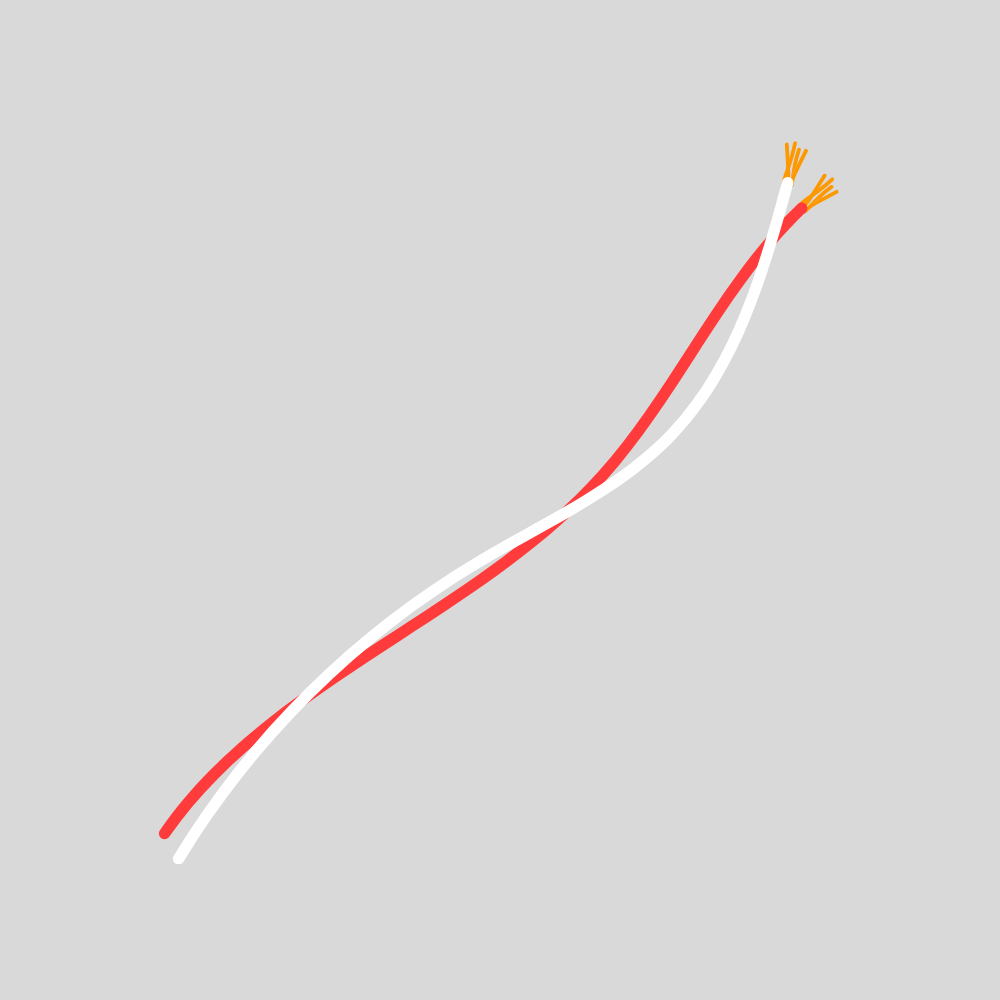
\includegraphics[width=\linewidth]{img/doppino_telefonico.png}
               \caption{{creata con \href{https://www.canva.com/}{Canva}}}
           \end{figure}
    \end{columns}
\end{frame}

\begin{frame}{MEZZI DI TRASMISSIONE DATI WIRED}
    \begin{columns}
        \column{.5\textwidth}
        \begin{alertblock}{CAVO ETHERNET}
            \begin{minipage}{0.97\linewidth}
                \justifying
                Formato da \textbf{quattro coppie} di filamenti di rame che aumentano moltissimo 
                la capacità di trasmissione del cavo rispetto al singolo doppino telefonico. 
                Alle estremità del cavo sono presenti connettori solitamente di standard \textbf{RJ45}. 
                Esistono differenti tipologie di cavi Ethernet, ognuna delle quali garantisce prestazioni 
                sempre maggiori (Cat5, Cat5e, Cat6, Cat7, Cat8).
            \end{minipage}
        \end{alertblock}
        \column{.5\textwidth}
           \begin{figure}
               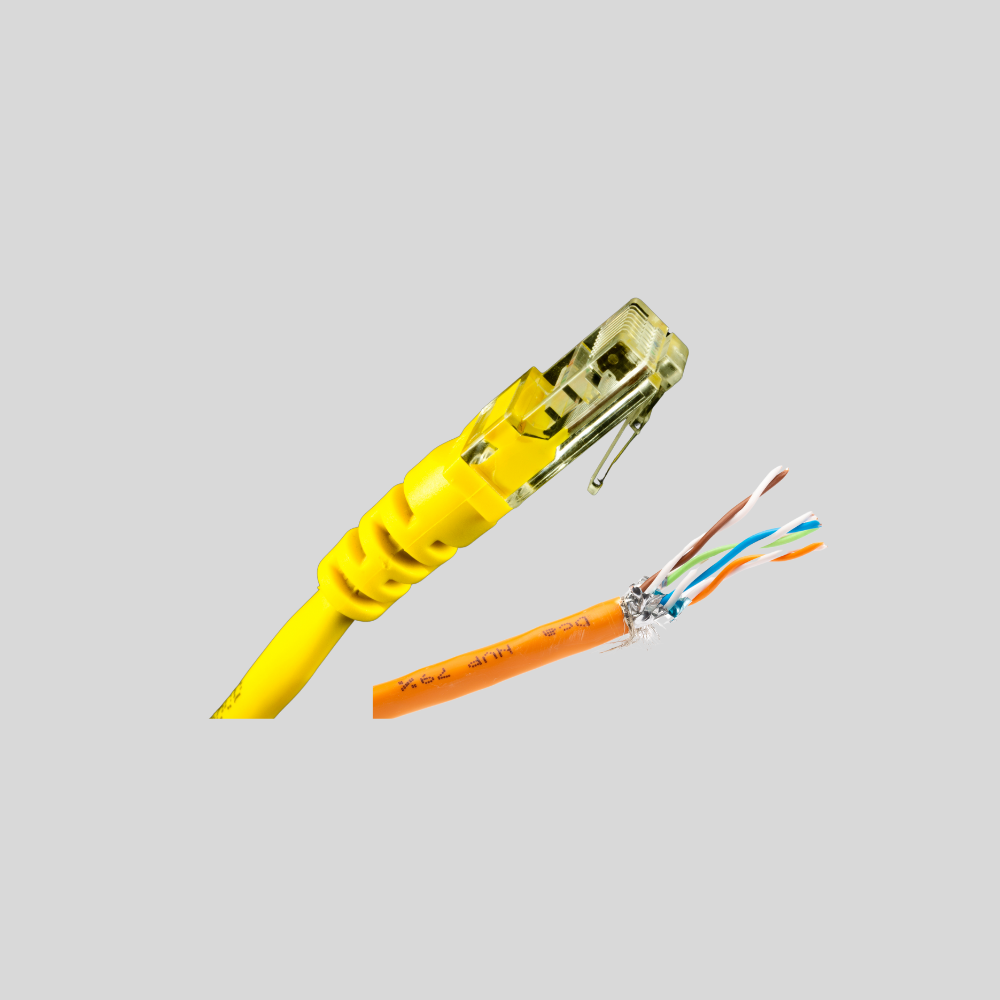
\includegraphics[width=\linewidth]{img/cavo_ethernet.png}
               \caption{{creata con \href{https://www.canva.com/}{Canva}}}
           \end{figure}
    \end{columns}
\end{frame}

\begin{frame}{MEZZI DI TRASMISSIONE DATI WIRED}
    \begin{columns}
        \column{.5\textwidth}
        \begin{alertblock}{FIBRA OTTICA}
            \begin{minipage}{0.97\linewidth}
                \justifying
                La Fibra Ottica, diversamente dai precedenti, non trasmette un segnale elettrico 
                su cavi di rame, ma trasmette un \textbf{segnale luminoso} che può potenzialmente raggiungere 
                la velocità della luce. La velocità e affidabilità del segnale di trasmissione è quindi 
                estremamente alta.
            \end{minipage}
        \end{alertblock}
        \column{.5\textwidth}
           \begin{figure}
               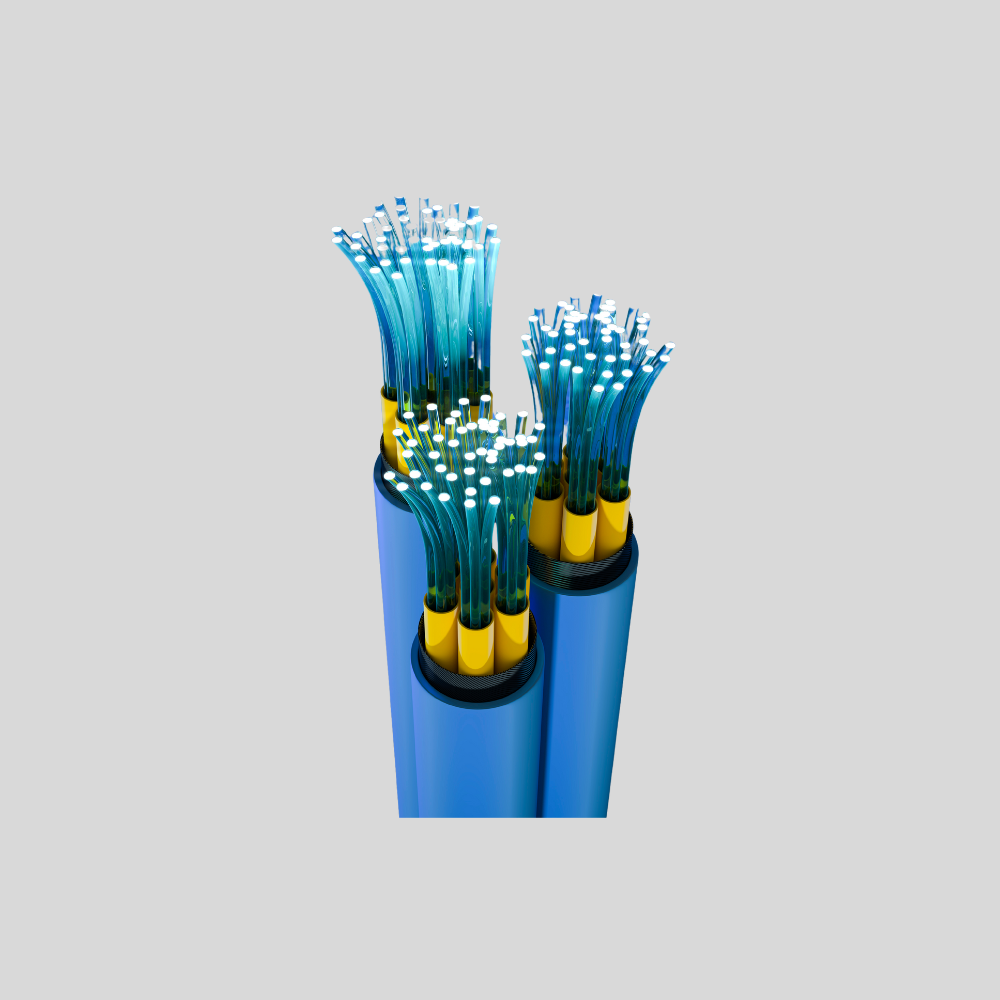
\includegraphics[width=\linewidth]{img/fibra_ottica.png}
               \caption{{creata con \href{https://www.canva.com/}{Canva}}}
           \end{figure}
    \end{columns}
\end{frame}

\begin{frame}{VELOCIT\'A DI TRASMISSIONE}
    \begin{alertblock}{DEFINIZIONE}
        \begin{minipage}{0.98\linewidth}
            \justifying
            In informatica e telecomunicazioni, \textbf{la velocità di trasmissione} 
            (detta anche \textbf{banda} o \textbf{bit-rate}), 
            è la grandezza indicante la quantità di informazione trasferita 
            attraverso un canale di comunicazione in un dato intervallo di tempo. 
            L'unità di misura associata è il bit per secondo (\textbf{bps}).
        \end{minipage}
    \end{alertblock}
\end{frame}

\begin{frame}{MEZZI DI TRASMISSIONE DATI (\href{https://www.fastweb.it/fastweb-plus/digital-magazine/velocita-connessione-internet-c-e-un-nuovo-record/}{record speed}, \href{https://misurainternet.it/misura-speedtest/}{speed test})}
    \begin{center}
        \centering
        \setlength{\tabcolsep}{30pt}
        \begin{tabular}{c|c}
            \textbf{TRASMISSIONE WIRED} & \textbf{BIT-RATE} \\
            \hline
            \hline
            \uncover<1->{Doppino telefonico (ADSL)} & \uncover<1->{fino a 24 Mbps (effettivo)} \\
            \hline
            \uncover<2->{Cavo Ethernet (LAN)} & \uncover<2->{4 Mbps - 40Gbps (teorico)} \\ 
            \hline
            \uncover<3->{Fibra Ottica FTTC (Cabinet)} & \uncover<3->{50 Mbps - 200 Mbps (effettivo)} \\
            \hline
            \uncover<4->{Fibra Ottica FTTH (Home)} & \uncover<4->{50 Mbps - 2,5Gbps (effettivo)} \\
            \hline
        \end{tabular}
    \end{center}
\end{frame}

\section{MEZZI DI TRASMISSIONE DATI WIRELESS}

\begin{frame}{FREQUENZA}
    \begin{alertblock}{DEFINIZIONE}
        \begin{minipage}{0.98\linewidth}
            \justifying
            In fisica \textbf{la frequenza} di un fenomeno che presenta un andamento costituito da 
            eventi che nel tempo si ripetono (identici o quasi identici), viene data dal numero 
            degli eventi che vengono ripetuti in una data unità di tempo. Nel misurare la frequenza 
            di onde elettromagnetiche (come le onde radio o la luce), la frequenza in \textbf{Hertz} è il numero 
            di cicli della forma d'onda ripetitiva per secondo. \textbf{Al crescere della frequenza} dell'onda radio corrisponde un \textbf{aumento della banda} 
            dati a disposizione ma, allo stesso tempo, \textbf{diminuisce la distanza} coperta dal segnale.
            Insomma, una sorta di coperta corta che bisogna saper adattare a seconda delle necessità, 
            così da massimizzare la resa del servizio di telecomunicazioni.
        \end{minipage}
    \end{alertblock}
\end{frame}

\begin{frame}{SPETTRO ELETTROMAGNETICO}
    \begin{columns}
        \column{.65\textwidth}
        \begin{figure}
            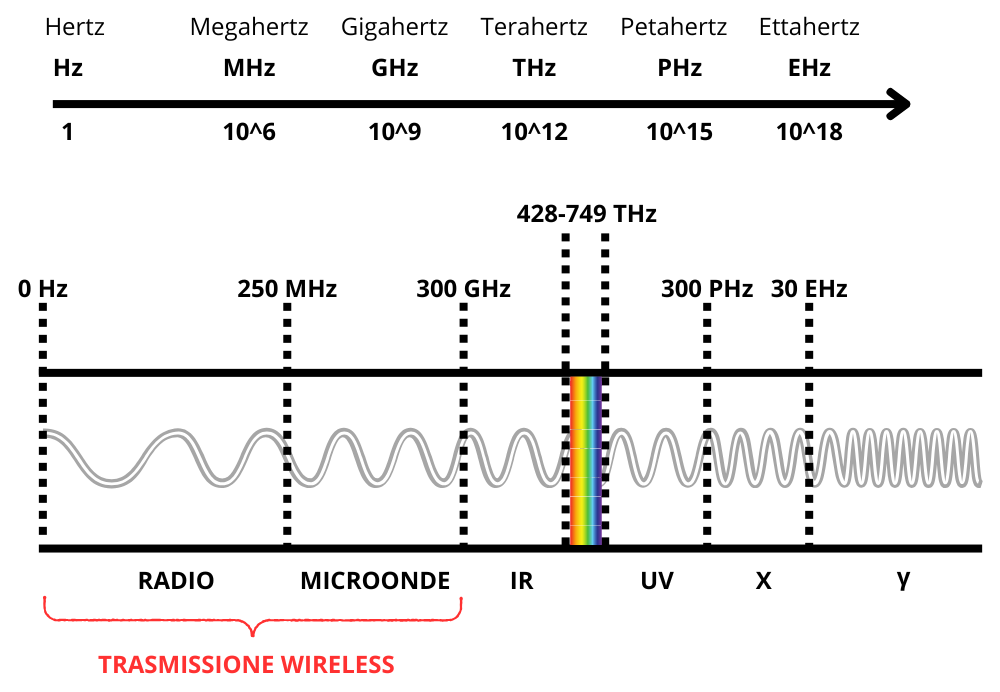
\includegraphics[width=\textwidth]{img/Spettro_Elettromagnetico.png}
            \caption{{creata con \href{https://www.canva.com/}{Canva}}}
        \end{figure}
    \end{columns}
\end{frame}

\begin{frame}{MEZZI DI TRASMISSIONE DATI (\href{https://newatlas.com/telecommunications/wireless-data-speed-record-938-gigabits-per-second/}{record speed})}
    \begin{center}
        \centering
        \setlength{\tabcolsep}{2pt}
        \begin{tabular}{c|c}
            \textbf{TRASMISSIONE WIRELESS} & \textbf{FREQUENZA} \\
            \hline
            \hline
            \uncover<1->{NFC (Near-Field Communication)} & \uncover<1->{13,56 MHz} \\
            \hline
            \uncover<2->{RFID (Radio-Frequency Identification)} & \uncover<2->{130 KHz - 13,56 MHz - 860 MHz} \\
            \hline
            \uncover<3->{Bluetooh} & \uncover<3->{2,4GHz} \\
            \hline
            \uncover<4->{Wi-Fi} & \uncover<4->{2,4GHz - 5GHz} \\
            \hline
            \uncover<5->{4G LTE} & \uncover<5->{800 MHz - 1800 MHz - 2600 MHz} \\
            \hline
            \uncover<6->{5G} & \uncover<6->{694:790 MHz - 3,6:3,8 GHz - 26,5:27,5 GHz} \\
            \hline
            \uncover<7->{GNSS(Global Navigation Satellite System)} & \uncover<7->{1,278 GHz - 1,575 GHz} \\
            \hline
        \end{tabular}  
    \end{center}
    \uncover<7->{
        \tiny{\textbf{Curiosità}}\\
        \tiny{\href{https://it.wikipedia.org/wiki/Sistema\_satellitare\_globale\_di\_navigazione}{GNSS attuali}} e 
        \tiny{\href{https://offerta-internet.it/satellitare}{Internet Satellitare}}
    }
\end{frame}

\section{MODALIT\'A DI TRASMISSIONE}

\begin{frame}{MODALIT\'A DI TRASMISSIONE}
    \begin{columns}
        \column{.5\textwidth}
        \begin{alertblock}{UNICAST}
            \begin{minipage}{0.96\linewidth}
                \justifying
                La comunicazione Unicast coinvolge la trasmissione dei dati da un mittente a \textbf{un 
                unico destinatario}. I dati vengono ricevuti da un unico dispositivo.\\
                ESEMPIO: trasmissione end-to-end.
            \end{minipage}
        \end{alertblock}
        \column{.5\textwidth}
           \begin{figure}
               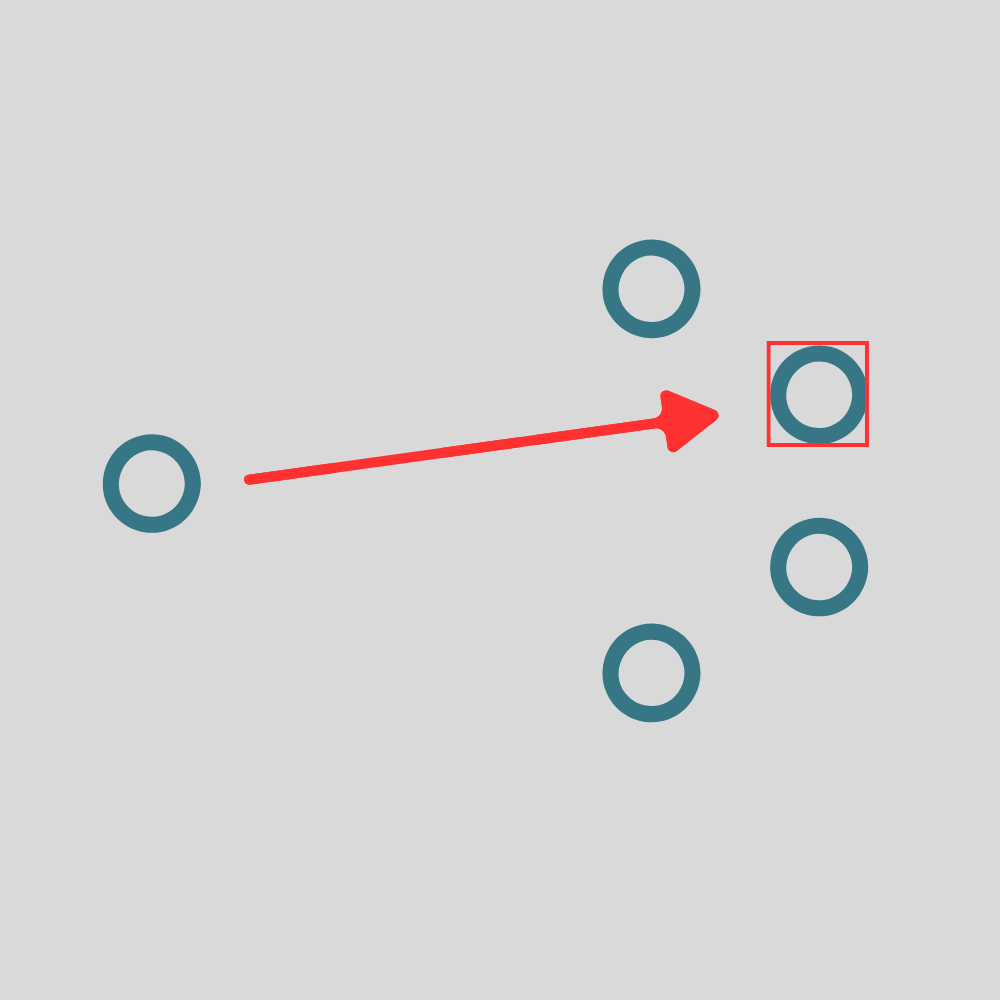
\includegraphics[width=\linewidth]{img/unicast.png}
               \caption{{creata con \href{https://www.canva.com}{Canva}}}
           \end{figure}
    \end{columns}
\end{frame}

\begin{frame}{MODALIT\'A DI TRASMISSIONE}
    \begin{columns}
        \column{.5\textwidth}
        \begin{alertblock}{MULTICAST}
            \begin{minipage}{0.96\linewidth}
                \justifying
                La comunicazione Multicast coinvolge la trasmissione dei dati da un mittente a \textbf{un 
                gruppo di destinatari}. I dati vengono ricevuti da uno o più dispositivi.\\
                ESEMPIO: videoconferenze private.
            \end{minipage}
        \end{alertblock}
        \column{.5\textwidth}
           \begin{figure}
               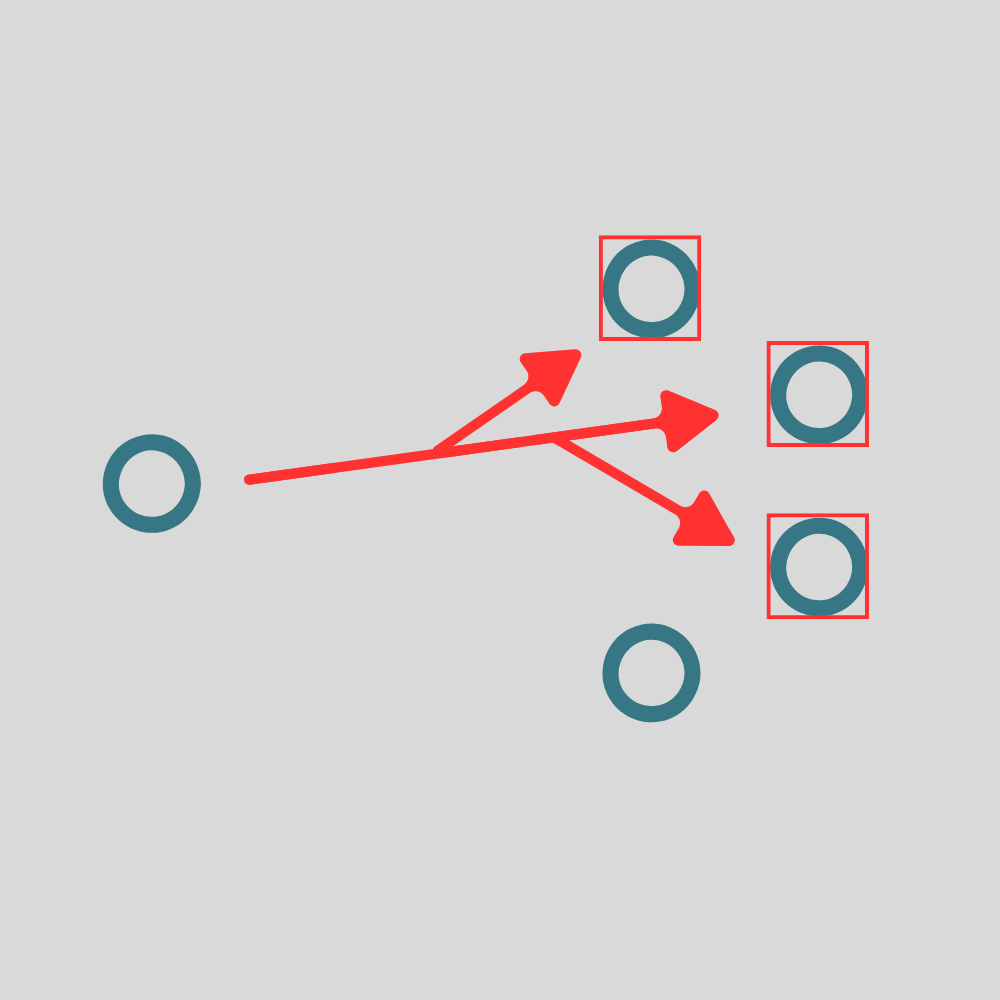
\includegraphics[width=\linewidth]{img/multicast.png}
               \caption{{creata con \href{https://www.canva.com}{Canva}}}
           \end{figure}
    \end{columns}
\end{frame}

\begin{frame}{MODALIT\'A DI TRASMISSIONE}
    \begin{columns}
        \column{.5\textwidth}
        \begin{alertblock}{ANYCAST}
            \begin{minipage}{0.96\linewidth}
                \justifying
                La comunicazione Anycast coinvolge la trasmissione dei dati da un mittente a \textbf{un 
                insieme di destinatari qualsiasi} all'interno di un gruppo. I dati vengono ricevuti da uno o più dispositivi.\\
                ESEMPIO: Routing Internet (i pacchetti sono instradati verso il nodo più vicino o più efficiente).                
            \end{minipage}
        \end{alertblock}
        \column{.5\textwidth}
           \begin{figure}
               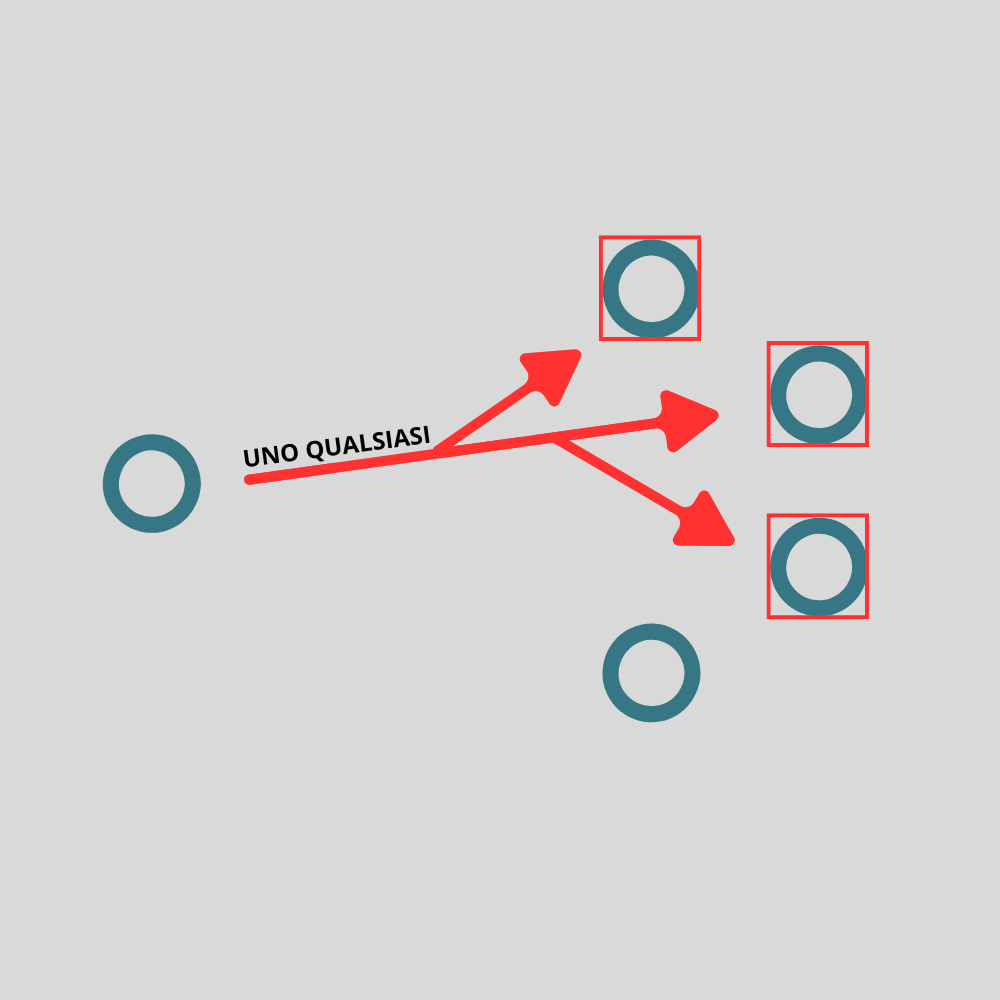
\includegraphics[width=\linewidth]{img/anycast.png}
               \caption{{creata con \href{https://www.canva.com}{Canva}}}
           \end{figure}
    \end{columns}
\end{frame}

\begin{frame}{MODALIT\'A DI TRASMISSIONE}
    \begin{columns}
        \column{.5\textwidth}
        \begin{alertblock}{BROADCAST}
            \begin{minipage}{0.96\linewidth}
                \justifying
                La comunicazione Broadcast coinvolge la trasmissione dei dati da un mittente a \textbf{tutti i 
                membri} di un gruppo. I dati vengono ricevuti da tutti i dispositivi.\\
                ESEMPIO: Messaggi di emergenza SOS.\\
                \bigskip
                \tiny{\textbf{Curiosità}}\\
                \tiny{\href{https://www.geopop.it/sos-significato-storia-segnale-universale-soccorso/}{Perchè SOS?}}
            \end{minipage}
        \end{alertblock}
        \column{.5\textwidth}
           \begin{figure}
               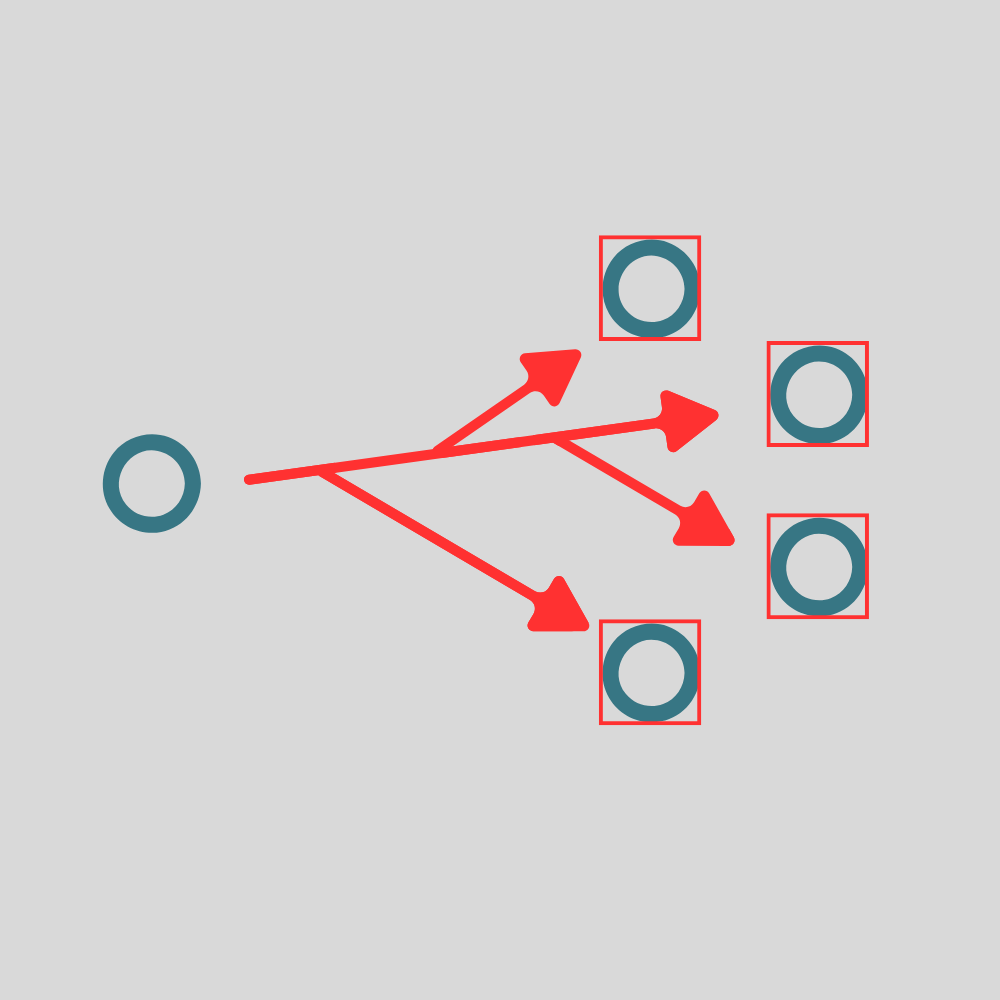
\includegraphics[width=\linewidth]{img/broadcast.png}
               \caption{{creata con \href{https://www.canva.com}{Canva}}}
           \end{figure}
    \end{columns}
\end{frame}

\section{MODALIT\'A DI TRASPORTO DELLA TRASMISSIONE}

\begin{frame}{MODALIT\'A DI TRASPORTO DELLA TRASMISSIONE}
    \begin{columns}
        \column{.5\textwidth}
        \begin{alertblock}{SIMPLEX}
            \begin{minipage}{0.96\linewidth}
                \justifying
                Le informazioni vengono trasmesse in un'\textbf{unica direzione}: da un mittente a un 
                destinatario, senza possibilità di risposta (nessun feedback).\\
                ESEMPI: televisione, radio.
            \end{minipage}
        \end{alertblock}
        \column{.5\textwidth}
           \begin{figure}
               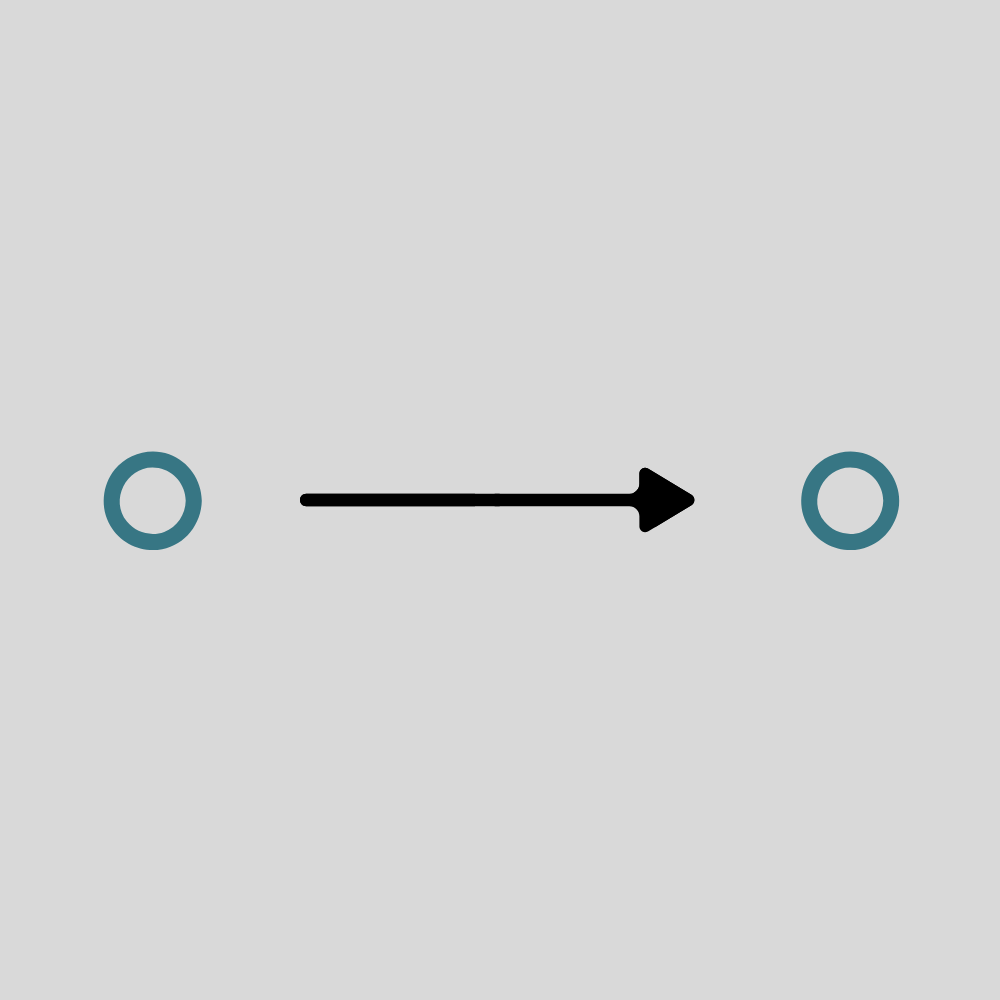
\includegraphics[width=\linewidth]{img/simplex.png}
               \caption{{creata con \href{https://www.canva.com}{Canva}}}
           \end{figure}
    \end{columns}
\end{frame}

\begin{frame}{MODALIT\'A DI TRASPORTO DELLA TRASMISSIONE}
    \begin{columns}
        \column{.5\textwidth}
        \begin{alertblock}{HALF-DUPLEX}
            \begin{minipage}{0.96\linewidth}
                \justifying
                Le informazioni vengono trasmesse in \textbf{entrambe le direzioni}: da un mittente a un 
                destinatario, ma non contemporaneamente. Lo scambio è alternato, il mittente e il destinatario si alternano
                nell'invio e nella ricezione delle informazioni.\\
                ESEMPIO: walkie-talkie.
            \end{minipage}
        \end{alertblock}
        \column{.5\textwidth}
           \begin{figure}
               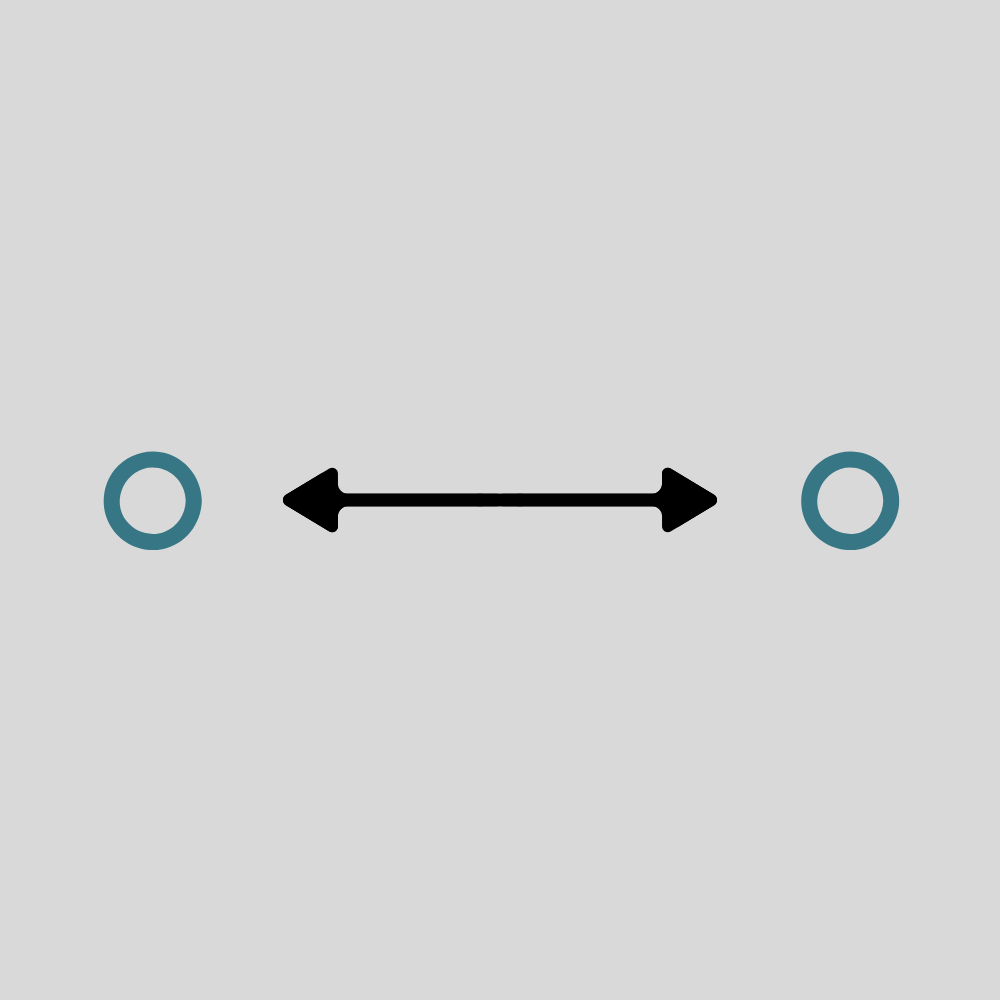
\includegraphics[width=\linewidth]{img/halfduplex.png}
               \caption{{creata con \href{https://www.canva.com}{Canva}}}
           \end{figure}
    \end{columns}
\end{frame}

\begin{frame}{MODALIT\'A DI TRASPORTO DELLA TRASMISSIONE}
    \begin{columns}
        \column{.5\textwidth}
        \begin{alertblock}{FULL-DUPLEX}
            \begin{minipage}{0.96\linewidth}
                \justifying
                Le informazioni vengono trasmesse in \textbf{entrambe le direzioni contemporaneamente} e senza interruzioni. 
                I mittenti possono essere contemporaneamente destinatari.\\
                ESEMPIO: telefono.
            \end{minipage}
        \end{alertblock}
        \column{.5\textwidth}
           \begin{figure}
               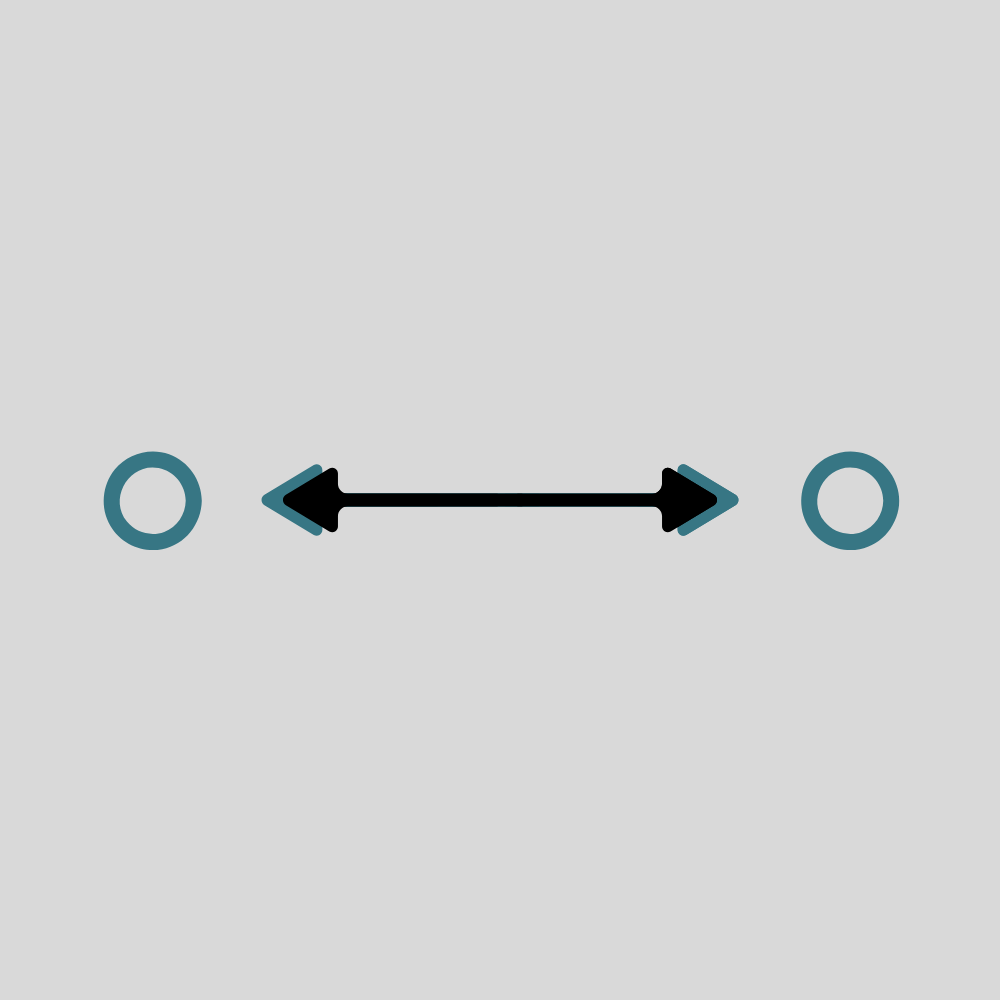
\includegraphics[width=\linewidth]{img/fullduplex.png}
               \caption{{creata con \href{https://www.canva.com}{Canva}}}
           \end{figure}
    \end{columns}
\end{frame}

\end{document}